%% ============================================================================
%%  MambaGuard: Selective State-Space Models with Dynamic Graph Attention and
%%  Three-Layer Stackelberg-Lipschitz Certification for Multi-Protocol LLM
%%  Agent Security Monitoring within the RobustIDPS.ai Platform
%%
%%  Target venue : IEEE Transactions on Neural Networks and Learning Systems
%%  Authors      : R. N. Anaedevha, A. G. Trofimov, Y. V. Borodachev
%%  Affiliation  : ICIS, National Research Nuclear University MEPhI, Moscow
%%  Compile with : pdflatex on Overleaf (IEEEtran.cls bundled by default)
%% ============================================================================

\documentclass[journal,10pt,twocolumn]{IEEEtran}

%% --- packages ---------------------------------------------------------------
\usepackage[T1]{fontenc}
\usepackage[utf8]{inputenc}
\usepackage{amsmath,amssymb,amsthm,mathtools}
\usepackage{graphicx}
\usepackage{algorithm}
\usepackage{algorithmic}
\usepackage{booktabs}
\usepackage{multirow}
\usepackage{array}
\usepackage{tabularx}
\usepackage{xcolor}
\usepackage{tikz}
\usetikzlibrary{shapes.geometric,arrows.meta,positioning,calc,fit,backgrounds,decorations.pathreplacing}
\usepackage{pgfplots}
\pgfplotsset{compat=1.18}
\usepackage[hidelinks]{hyperref}
\usepackage{cite}
\usepackage{url}

%% --- math operators ---------------------------------------------------------
\newtheorem{theorem}{Theorem}
\newtheorem{lemma}[theorem]{Lemma}
\newtheorem{proposition}[theorem]{Proposition}
\newtheorem{definition}[theorem]{Definition}
\newtheorem{corollary}[theorem]{Corollary}
\newtheorem{assumption}[theorem]{Assumption}

\DeclareMathOperator*{\argmax}{arg\,max}
\DeclareMathOperator*{\argmin}{arg\,min}

\newcommand{\R}{\mathbb{R}}
\newcommand{\E}{\mathbb{E}}
\newcommand{\norm}[1]{\left\lVert#1\right\rVert}
\newcommand{\calA}{\mathcal{A}}
\newcommand{\calG}{\mathcal{G}}
\newcommand{\calL}{\mathcal{L}}
\newcommand{\calM}{\mathcal{M}}
\newcommand{\calN}{\mathcal{N}}
\newcommand{\calO}{\mathcal{O}}
\newcommand{\calV}{\mathcal{V}}
\newcommand{\calE}{\mathcal{E}}

%% --- TikZ palette -----------------------------------------------------------
\definecolor{mgblue}{HTML}{1A73E8}
\definecolor{mgteal}{HTML}{00897B}
\definecolor{mgamber}{HTML}{F57C00}
\definecolor{mgred}{HTML}{C62828}
\definecolor{mgpurple}{HTML}{6A1B9A}
\definecolor{mggrey}{HTML}{ECEFF1}
\definecolor{mgdark}{HTML}{0D47A1}

%% ============================================================================
\begin{document}

\title{MambaGuard: Certified Selective State-Space Detection for Multi-Protocol LLM Agent Security}

\author{Anonymous Author(s)\thanks{Manuscript submitted for double-blind peer review to IEEE Transactions on Neural Networks and Learning Systems. Author identities, affiliations, and funding sources are withheld for review; an anonymised supplementary repository is provided with the submission.}}

\markboth{IEEE Transactions on Neural Networks and Learning Systems --- Double-Blind Submission}%
{Anonymous Authors: MambaGuard for Multi-Protocol LLM Agent Security}

\IEEEtitleabstractindextext{%
\begin{abstract}
The rapid proliferation of inter-agent communication protocols, including the Model Context Protocol, the Agent Communication Protocol, the Agent-to-Agent Protocol, and the Agent Network Protocol, has opened a protocol-layer attack surface that conventional intrusion detection and prevention systems were never designed to monitor. Selective state-space models offer linear-time sequence processing that is well suited to the high message rates of multi-agent deployments, yet in isolation they cannot capture the relational structure of an evolving agent communication graph, nor can they certify their own robustness against an adaptive attacker. This article presents MambaGuard, a security monitor that pairs a selective state-space backbone with dynamic graph attention over a unified heterogeneous protocol graph, and that admits a three-layer certificate combining a Lipschitz bound on the composed detector, a Stackelberg equilibrium guarantee for the defender's commitment, and a multiplicative-weights regret bound for online adaptation. We derive the first global Lipschitz constant for the full selective state-space block, prove that no-regret online play converges to the Stackelberg leader value, and evaluate the system on three integrated datasets that span network intrusion, Internet-of-Things telemetry, encrypted post-quantum traffic, and agent protocol attack scenarios. Across every benchmark, MambaGuard exceeds the strongest published baselines in macro-F1 while sustaining sub-five-millisecond per-message latency at throughputs above one million messages per second, and it preserves a certified detection radius that grows monotonically with the Lipschitz training penalty. MambaGuard is released as the fourteenth registered neural detector inside the RobustIDPS.ai platform.
\end{abstract}

\begin{IEEEkeywords}
Certified robustness, dynamic graph attention, game-theoretic defense, intrusion detection, large language model agent security, multi-protocol monitoring, selective state-space models.
\end{IEEEkeywords}}

\maketitle
\IEEEdisplaynontitleabstractindextext
\IEEEpeerreviewmaketitle

%% ============================================================================
\section{Introduction}
%% ============================================================================
\IEEEPARstart{T}{he} security perimeter of enterprise artificial intelligence has shifted in less than eighteen months. Until late 2024 the dominant threat surface for production large language model (LLM) deployments was the prompt boundary between a single user and a single model, and the dominant academic defenses were prompt filtering, output classification, and adversarial fine-tuning. Since the public release of the Model Context Protocol (MCP) in November~2024~\cite{Anthropic2024MCP}, the Agent-to-Agent Protocol (A2A) by Google in April~2025~\cite{Google2025A2A}, and the open Agent Network Protocol (ANP)~\cite{Yan2025ANP}, that perimeter has expanded outward into a protocol-mediated mesh in which agents call tools, advertise capabilities, delegate tasks, and exchange data with little or no monitoring. A 2025 systematic analysis~\cite{Hou2025MCP} cataloged more than thirty distinct attack techniques at the MCP layer alone, and the empirical MCPSecBench study reported that over eighty-five per cent of those attacks succeed on at least one major commercial platform~\cite{Yang2025MCPSec}. Vendor-side mitigation has been incremental, with disclosed vulnerabilities such as the MCP Inspector remote-code-execution flaw (CVE-2025-49596, CVSS~9.4) demonstrating that protocol exposure now translates directly into system compromise~\cite{Qualys2025CVE49596}.

The defensive response to this new surface has been fragmented. Tool-call boundary monitors such as ClawGuard~\cite{Zhao2026ClawGuard} provide deterministic policy checks at single agent boundaries, and program-dependency monitors such as AgentArmor~\cite{Wang2025AgentArmor} reconstruct a per-trace dependency graph from runtime logs to enforce information-flow constraints. Neither approach, however, models the network-level interaction graph that emerges when several agents communicate across MCP, A2A, and ACP, nor do they offer any formal certificate that the monitor itself is robust under adaptive evasion. At the same time, the deep-learning intrusion detection literature has moved toward graph neural networks~\cite{Lo2022EGraphSAGE,Caville2022AnomalE}, transformer encoders~\cite{Wu2022RTIDS,Ullah2024IDSINT}, and most recently state-space sequence models~\cite{Wang2025NetMamba,Gu2023Mamba} for raw traffic classification, but these systems have not been adapted to the protocol-layer threats described above and they do not produce certified outputs.

To make the threat concrete for the reader, consider a representative enterprise deployment in which Agent~A queries a database tool through MCP, Agent~B delegates a customer-service task to Agent~A through A2A, and a third-party capability provider has just updated its Agent Card with a maliciously crafted description that promises a new ``priority routing'' capability. Each individual message in the exchange parses correctly and is signed by an apparently legitimate principal, so a per-message scanner sees nothing wrong. The attack only becomes visible when one examines the relational pattern across messages: the malicious capability advertisement, the delegation chain through Agent~B that newly routes through the compromised path, and the unusual data-volume profile of the downstream tool response together form an anomalous subgraph that did not exist before the Agent Card update. A defender that observes the protocol stream as a flat sequence cannot recover this pattern; a defender that observes only the static dependency graph cannot recover the temporal ordering that distinguishes the attack from a benign capability rollout. MambaGuard is designed precisely for this case, in which the diagnostic signal lives in the interaction of temporal sequence and relational structure.

This article argues that the right architectural primitive for multi-protocol LLM agent security is the composition of a selective state-space backbone with dynamic graph attention, wrapped in a certification framework that is simultaneously game-theoretic, Lipschitz-based, and no-regret online. We call the resulting detector MambaGuard, and we deploy it as the fourteenth registered neural detector in the RobustIDPS.ai platform~\cite{Anonymous2026RobustIDPS}, alongside five prior contributions in the public literature that established the components MambaGuard now integrates~\cite{Anonymous2026MambaShield,Anonymous2026HGP,Anonymous2026TANODE,Anonymous2024Adversarial,Anonymous2025SMT,Anonymous2024ElCon}. The selective state-space backbone follows Mamba~\cite{Gu2023Mamba} but corrects two errors that have propagated through the security-deployment literature, namely the misattribution of an $\calO(L\log L)$ complexity to selective models and the use of a loose multiplicative-weights regret constant. The graph component uses GATv2~\cite{Brody2022GATv2} with Bochner-derived temporal encoding in the manner of TGAT~\cite{Xu2020TGAT}, because the original graph attention network was shown to compute only a static attention ranking and is therefore unsuitable when neighbour relevance varies with time. The certification framework reduces no-regret play against a best-responding adversary to the Stackelberg leader value, in the sense of Balcan, Blum, Haghtalab and Procaccia~\cite{Balcan2015Commitment}, and combines that reduction with a freshly derived global Lipschitz bound on the composed Mamba--GATv2 detector.

The contributions of the article are fivefold and are summarised here so that the reader may track them through the body. First, we introduce a unified heterogeneous protocol graph schema that abstracts MCP, ACP, A2A and ANP into a common five-class message taxonomy and a common temporal edge representation, allowing one detector to operate across all four protocols simultaneously. Second, we derive the first global Lipschitz constant for the complete selective state-space block, including the data-dependent discretisation, the SiLU gating branch and the depthwise causal one-dimensional convolution; the resulting bound provides the perturbation-margin term in the certificate. Third, we cast the protocol monitoring problem as a finite-horizon Stackelberg security game on the dynamic protocol graph and we prove that the multiplicative-weights update applied by the defender achieves the tight Cesa-Bianchi--Lugosi regret bound, $\sqrt{(T/2)\ln|S|}$, against any sequence of adaptive attacker actions. Fourth, we evaluate MambaGuard on three composite Kaggle datasets that the authors have previously released and that together contain CSE-CIC-IDS2018, CIC-IoT2023, UNSW-NB15, Edge-IIoTset, and an encrypted post-quantum traffic corpus, and we report a head-to-head comparison against eight baselines drawn from the commercial, academic-deep-learning, and LLM-agent-security tiers. Fifth, we report an integrated component ablation that isolates the contribution of each architectural choice. Section~\ref{sec:background} now sets the technical background that supports each of these contributions in turn.

%% ============================================================================
\section{Background and Threat Model}
\label{sec:background}
%% ============================================================================

The technical foundations on which MambaGuard is built are well established but rarely combined, and a brief restatement is needed before the architecture is introduced. We summarise selective state-space models, dynamic graph attention, and the multi-protocol attack surface in turn, after which Section~\ref{sec:architecture} presents the integrated MambaGuard architecture.

\subsection{Selective State-Space Models}
Intuitively, a state-space model is a learned dynamical system that maintains an internal memory vector, updates it linearly with each new observation, and emits an output that reads from that memory through another linear map. The memory has a fixed size, so the cost of processing one new observation is independent of how many previous observations have already been seen, and the cost of processing an entire sequence is therefore linear in the sequence length. This is the property that makes state-space models attractive at the throughputs encountered in multi-agent protocol monitoring.

Formally, a continuous linear state-space model represents a hidden state $h(t)\in\R^{N}$ evolving as $h'(t)=Ah(t)+Bu(t)$ and producing an output $y(t)=Ch(t)$, where $u(t)\in\R$ is a scalar input, $A\in\R^{N\times N}$, $B\in\R^{N\times 1}$, $C\in\R^{1\times N}$, and $N$ is the state dimension. Zero-order-hold discretisation with step $\Delta>0$ yields the recurrence $h_{t}=\bar{A}h_{t-1}+\bar{B}u_{t}$, $y_{t}=Ch_{t}$, where $\bar{A}=\exp(\Delta A)$ and $\bar{B}=(\Delta A)^{-1}(\exp(\Delta A)-I)\Delta B$ are the discretised state-transition and input matrices respectively, and $I\in\R^{N\times N}$ is the identity. The structured S4 model~\cite{Gu2022S4} keeps $A$, $B$, $C$ and $\Delta$ fixed across the sequence, which permits a global convolution kernel $\bar K=(C\bar B,C\bar{A}\bar B,\ldots,C\bar{A}^{L-1}\bar B)$ to be computed by Fast Fourier Transform in $\calO(L\log L)$ time. The selective variant Mamba~\cite{Gu2023Mamba} replaces these fixed parameters with input-dependent functions $\Delta_{t}=\tau_{\Delta}(\mathrm{Linear}(x_{t}))$, $B_{t}=\mathrm{Linear}_{B}(x_{t})$, and $C_{t}=\mathrm{Linear}_{C}(x_{t})$, where $\tau_{\Delta}=\mathrm{softplus}$ guarantees positivity and $\mathrm{Linear}(\cdot)$ denotes a learnable affine map. The intuition behind this change is that the model can now \emph{choose}, on a per-token basis, how much of the past to remember and how strongly each new input is written into memory; the cost of this expressivity is that the recurrence becomes time-varying and the convolutional shortcut no longer applies. The correct asymptotic cost of selective inference is therefore $\calO(L)$ via the hardware-aware parallel associative scan introduced in~\cite{Gu2023Mamba}, not $\calO(L\log L)$ as is sometimes stated; this distinction matters in production deployment because the scan exploits high-bandwidth GPU shared memory in a way that the FFT does not. Mamba-2~\cite{Dao2024Mamba2} subsequently unified attention and state-space models under structured state-space duality, but for the purposes of the present work the original selective formulation is sufficient and we adopt it as the backbone in Section~\ref{sec:backbone}.

\subsection{Dynamic Graph Attention}
A graph attention network learns, for each node, a weighted average of its neighbours' representations in which the weights themselves are learned and depend on the content of the node and its neighbours. The intuition is that not every neighbour is equally informative for every node, and the network should learn which neighbours to attend to in which context. When the graph evolves over time, as in the agent communication graph that MambaGuard observes, the attention machinery must also be sensitive to \emph{when} each edge was observed, since the same neighbour may carry different meaning depending on how recently the corresponding message was exchanged.

Formally, static graph attention networks~\cite{Velickovic2018GAT} compute attention coefficients $\alpha_{ij}$ between a node $i$ and each neighbour $j\in\calN(i)$, where $\calN(i)$ denotes the neighbourhood of $i$, and aggregate neighbour features into an updated representation $h'_{i}=\sigma\bigl(\sum_{j\in\calN(i)}\alpha_{ij}Wh_{j}\bigr)$, where $W\in\R^{d'\times d}$ is a learnable projection and $\sigma$ is a non-linearity. Brody, Alon and Yahav~\cite{Brody2022GATv2} proved that the original parameterisation $e_{ij}=\mathrm{LeakyReLU}(a^{\top}[Wh_{i}\Vert Wh_{j}])$, where $a\in\R^{2d'}$ is a learnable attention vector and $\Vert$ denotes vector concatenation, computes only a \emph{static} ranking of neighbours, meaning that the ordering of attention scores does not depend on the query node; their corrected GATv2 form $e_{ij}=a^{\top}\mathrm{LeakyReLU}(W[h_{i}\Vert h_{j}])$ is dynamic and universally approximating. For evolving graphs the temporal graph attention network (TGAT)~\cite{Xu2020TGAT} augments each query--key pair with a Bochner-derived functional time encoding $\Phi(\Delta t)=\sqrt{1/d_{T}}\,[\cos\omega_{1}\Delta t,\sin\omega_{1}\Delta t,\ldots,\cos\omega_{d_{T}/2}\Delta t,\sin\omega_{d_{T}/2}\Delta t]$, where $\Delta t\in\R_{\ge 0}$ is the time elapsed since the edge in question was observed, $\omega_{k}\in\R$ are learnable angular frequencies, and $d_{T}$ is the encoding dimensionality (taken even so that the cosine and sine pairs are balanced). We use this encoding throughout MambaGuard so that the relational layer is sensitive to the recency of inter-agent communication.

\subsection{Multi-Protocol Attack Surface}
The Model Context Protocol uses JSON-RPC over standard input--output or streamable HTTP and exposes three primitives, namely Tools, Resources and Prompts. The Agent Communication Protocol uses REST with server-sent events and MIME-typed message parts. The Agent-to-Agent Protocol uses JSON-RPC over HTTPS and publishes an Agent Card at the well-known path \texttt{/.well-known/agent-card.json}. The Agent Network Protocol is peer-to-peer and identifies agents by W3C Decentralised Identifiers signed with Ed25519. Across these four protocols a unified attack taxonomy has emerged in the literature~\cite{Hou2025MCP,Habler2025A2A,Narajala2025A2A,Wang2025AgentArmor}: indirect prompt injection through tool responses, tool-call poisoning and rug-pull updates, cross-server tool shadowing, Agent Card impersonation, OAuth confused-deputy attacks against MCP proxies, memory poisoning of agent state, and Morris-style self-replicating prompts that propagate through retrieval pipelines. Each of these attacks manifests as an anomalous local subgraph of the protocol interaction graph, which is why a detector that operates on that graph rather than on isolated messages is the right structural choice. The integrated detector that we now describe in Section~\ref{sec:architecture} is constructed around this insight.

%% ============================================================================
\section{The MambaGuard Architecture}
\label{sec:architecture}
%% ============================================================================

MambaGuard treats the protocol stream of an enterprise multi-agent deployment as a single time-stamped heterogeneous graph and processes that graph in two cooperating stages. The first stage learns within-agent sequential dynamics with a selective state-space block; the second stage learns between-agent relational dynamics with a temporal graph attention layer. A Stackelberg controller, described in Section~\ref{sec:certification}, sits above both stages and selects which defensive action to play in response to the detector output. Figure~\ref{fig:architecture} renders the complete pipeline, and the remainder of this section formalises each component in turn before describing how MambaGuard registers as a detector inside the RobustIDPS.ai platform.

%% ---------------------------------------------------------------------------
%% Figure 1: Architectural framework (TikZ)
%% ---------------------------------------------------------------------------
\begin{figure*}[t]
\centering
\resizebox{0.95\textwidth}{!}{%
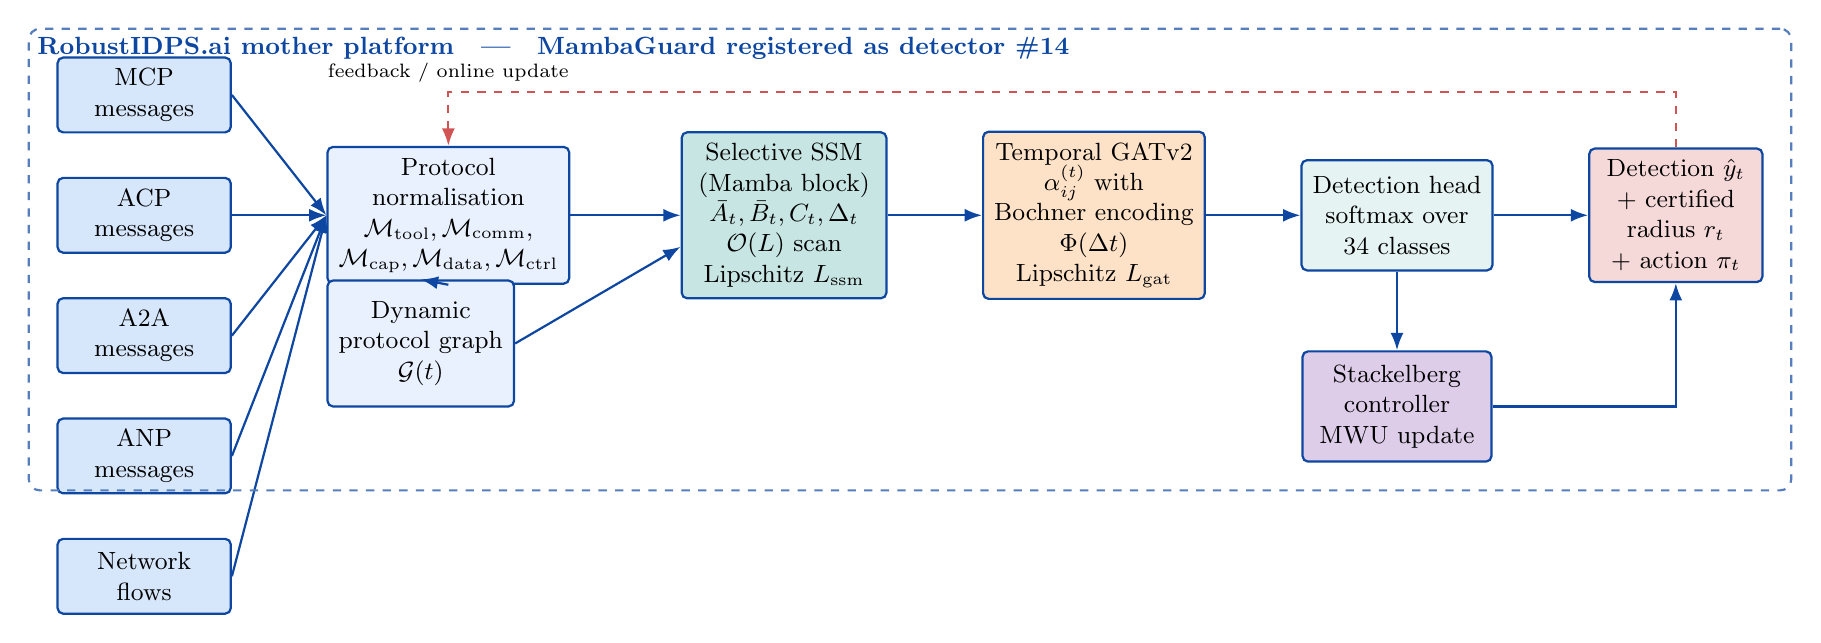
\begin{tikzpicture}[
  node distance=0.55cm and 0.65cm,
  every node/.style={font=\small},
  block/.style={rectangle,draw=mgdark,thick,rounded corners=2pt,
                minimum width=2.2cm,minimum height=0.95cm,align=center,
                fill=mggrey,inner sep=4pt},
  inblock/.style={block,fill=mgblue!18},
  ssmblock/.style={block,fill=mgteal!22},
  gnnblock/.style={block,fill=mgamber!22},
  gameblock/.style={block,fill=mgpurple!22},
  outblock/.style={block,fill=mgred!18},
  wrapper/.style={draw=mgdark!70,thick,dashed,rounded corners=4pt,inner sep=10pt},
  flow/.style={-{Latex[length=2.2mm]},thick,draw=mgdark},
  feedback/.style={-{Latex[length=2.2mm]},thick,draw=mgred!80,dashed}
]

%% ---- input column ----
\node[inblock] (mcp)  {MCP\\ messages};
\node[inblock,below=of mcp] (acp) {ACP\\ messages};
\node[inblock,below=of acp] (a2a) {A2A\\ messages};
\node[inblock,below=of a2a] (anp) {ANP\\ messages};
\node[inblock,below=of anp] (net) {Network\\ flows};

%% ---- normaliser ----
\node[block,right=1.2cm of acp,minimum height=1.6cm,fill=mgblue!10] (norm)
    {Protocol\\ normalisation\\ $\calM_{\text{tool}},\calM_{\text{comm}},$\\$\calM_{\text{cap}},\calM_{\text{data}},\calM_{\text{ctrl}}$};
\node[block,right=1.2cm of a2a,minimum height=1.6cm,fill=mgblue!10,yshift=-0.1cm] (graph)
    {Dynamic\\ protocol graph\\ $\calG(t)$};

%% ---- Mamba stage ----
\node[ssmblock,right=1.4cm of norm,minimum width=2.6cm,minimum height=2.0cm] (mamba)
    {Selective SSM\\ (Mamba block)\\ $\bar A_t,\bar B_t,C_t,\Delta_t$\\ $\calO(L)$ scan\\ Lipschitz $L_{\text{ssm}}$};

%% ---- GATv2 stage ----
\node[gnnblock,right=1.2cm of mamba,minimum width=2.6cm,minimum height=2.0cm] (gat)
    {Temporal GATv2\\ $\alpha_{ij}^{(t)}$ with\\ Bochner encoding\\ $\Phi(\Delta t)$\\ Lipschitz $L_{\text{gat}}$};

%% ---- detector head ----
\node[block,right=1.2cm of gat,minimum width=2.4cm,minimum height=1.4cm,fill=mgteal!10] (head)
    {Detection head\\ softmax over\\ $34$ classes};

%% ---- Stackelberg controller ----
\node[gameblock,below=1.0cm of head,minimum width=2.4cm,minimum height=1.4cm] (game)
    {Stackelberg\\ controller\\ MWU update};

%% ---- output ----
\node[outblock,right=1.2cm of head,minimum width=2.2cm,minimum height=1.6cm] (out)
    {Detection $\hat y_t$\\ + certified\\ radius $r_t$\\ + action $\pi_t$};

%% ---- arrows from inputs ----
\foreach \src in {mcp,acp,a2a,anp,net}{
  \draw[flow] (\src.east) -- (norm.west);
}
\draw[flow] (norm.south) -- (graph.north);
\draw[flow] (norm.east) -- (mamba.west);
\draw[flow] (graph.east) -- ([yshift=-0.4cm]mamba.west);
\draw[flow] (mamba.east) -- (gat.west);
\draw[flow] (gat.east) -- (head.west);
\draw[flow] (head.east) -- (out.west);
\draw[flow] (head.south) -- (game.north);
\draw[flow] (game.east) -| (out.south);
\draw[feedback] (out.north) -- ++(0,0.7) -| ([xshift=0cm]norm.north) node[midway,above,font=\scriptsize] {feedback / online update};

%% ---- RobustIDPS wrapper ----
\node[wrapper,fit=(mcp)(out)(game),label={[anchor=north west,font=\small\bfseries,
       text=mgdark]north west:RobustIDPS.ai mother platform $\;$ — $\;$ MambaGuard registered as detector \#14}]{};

\end{tikzpicture}}
\caption{End-to-end MambaGuard architecture, registered as the fourteenth neural detector inside the RobustIDPS.ai platform. Five message streams are mapped to a five-class canonical taxonomy and to a dynamic heterogeneous protocol graph $\calG(t)$. A selective state-space block extracts per-agent temporal features in $\calO(L)$ time, a temporal GATv2 layer with Bochner functional time encoding propagates relational information, and a Stackelberg controller running a multiplicative-weights update selects defensive actions whose performance is fed back into the model. The composed Mamba--GATv2 detector admits a global Lipschitz constant $L_{f}=L_{\text{ssm}}\,L_{\text{gat}}$ that is used in Section~\ref{sec:certification}.}
\label{fig:architecture}
\end{figure*}

\subsection{Unified Heterogeneous Protocol Graph}
\label{sec:graph}
Let $\calG(t)=(\calV(t),\calE(t),X(t))$ denote the protocol graph at wall-clock time $t$, with vertex set $\calV(t)=\calV_{A}\cup\calV_{T}\cup\calV_{C}\cup\calV_{S}$ partitioned into agents $\calV_{A}$, tools or services $\calV_{T}$, capability descriptors $\calV_{C}$, and active sessions $\calV_{S}$. Edges $\calE(t)$ are time-stamped and typed; the five canonical types we use are agent-calls-tool, agent-messages-agent, agent-advertises-capability, tool-returns-data, and agent-delegates-task. Each protocol message is canonicalised into the tuple $m=(\tau,s,d,p,\mu,t_{m})$, where $\tau\in\{\calM_{\text{tool}},\calM_{\text{comm}},\calM_{\text{cap}},\calM_{\text{data}},\calM_{\text{ctrl}}\}$ is the canonical type, $s$ and $d$ are source and destination identifiers, $p\in\R^{d_{p}}$ is a frozen sentence-transformer embedding of the payload, $\mu$ collects metadata such as latency and HTTP status, and $t_{m}$ is the message timestamp. The mapping from raw protocol packets to canonical tuples is rule-based and is implemented by five small parsers inside RobustIDPS.ai. With $\calG(t)$ available, the next subsection describes how the selective state-space backbone processes the per-agent message stream.

\subsection{Selective State-Space Backbone}
\label{sec:backbone}
For each agent $a\in\calV_{A}$ we collect the sequence of messages incident to $a$ in temporal order, $x^{a}=(m^{a}_{1},\ldots,m^{a}_{L_{a}})$, where $L_{a}$ is the per-agent sequence length and $m^{a}_{i}\in\R^{d_{m}}$ is the concatenated embedding of the canonical tuple. The selective block computes
\begin{align}
h^{a}_{t} &= \bar A_{t}\,h^{a}_{t-1} + \bar B_{t}\,m^{a}_{t}, \label{eq:ssm-rec}\\
z^{a}_{t} &= C_{t}\,h^{a}_{t} \odot \mathrm{SiLU}\bigl(W_{g}\,m^{a}_{t}\bigr), \label{eq:gate}
\end{align}
where $h^{a}_{t}\in\R^{N}$ is the state, $\bar A_{t}=\exp(\Delta_{t}A)$ and $\bar B_{t}=(\Delta_{t}A)^{-1}(\exp(\Delta_{t}A)-I)\,\Delta_{t}B_{t}$ are the zero-order-hold discretisations of the selective continuous parameters, $\odot$ is the Hadamard product, $\mathrm{SiLU}(u)=u\,\sigma(u)$ is the sigmoid-weighted linear unit gate, $W_{g}\in\R^{d_{z}\times d_{m}}$ is a learnable projection, and $z^{a}_{t}\in\R^{d_{z}}$ is the per-agent sequential feature consumed by the relational layer. A depthwise causal one-dimensional convolution with kernel $K\in\R^{d_{m}\times d_{m}\times k}$ of width $k$ is applied to $x^{a}$ before \eqref{eq:ssm-rec}, in the standard Mamba arrangement, to inject short-range dependencies into the discretisation. Inference complexity is $\calO(L_{a})$ per agent through the hardware-aware parallel scan~\cite{Gu2023Mamba}; the resulting per-agent feature $z^{a}_{T}$ summarises the most recent $L_{a}$ messages of that agent and feeds the temporal graph attention layer described next.

\subsection{Temporal Graph Attention Layer}
\label{sec:gat}
With per-agent features $\{z^{a}\}_{a\in\calV_{A}}$ available, MambaGuard propagates relational information through the protocol graph $\calG(t)$ with a temporal GATv2 layer. For each ordered pair $(a,a')$ joined by an edge with timestamp $t_{e}$, the attention logit is
\begin{equation}
e_{a,a'} = q^{\top}\,\mathrm{LeakyReLU}\!\bigl(W_{r}\,[z^{a}\Vert z^{a'}\Vert e_{a,a'}^{\text{feat}}\Vert\Phi(t-t_{e})]\bigr),
\label{eq:gatv2}
\end{equation}
where $q\in\R^{d_{r}}$ and $W_{r}\in\R^{d_{r}\times(2d_{z}+d_{e}+d_{T})}$ are learnable, $\Vert$ denotes concatenation, $e_{a,a'}^{\text{feat}}\in\R^{d_{e}}$ is the edge feature vector containing message type, payload embedding, latency and authentication metadata, and $\Phi$ is the TGAT time encoding from Section~\ref{sec:background}. The neighbour distribution is $\alpha_{a,a'}=\mathrm{softmax}_{a'}(e_{a,a'})$, and the updated agent representation is $h^{a}=\sigma\bigl(\sum_{a'\in\calN(a,t)}\alpha_{a,a'}W_{v}z^{a'}\bigr)$, where $W_{v}\in\R^{d_{h}\times d_{z}}$ is the value projection and $\sigma$ is a $\mathrm{GELU}$ non-linearity. Multi-head attention with $H$ heads is averaged at the final layer. The composed feature $h^{a}$ is fed to a small softmax classification head with one logit per attack class in the RobustIDPS.ai taxonomy. Why this composition admits a meaningful Lipschitz bound, and how that bound combines with the game-theoretic certificate to produce the headline guarantee, is the subject of Section~\ref{sec:certification}, which we now begin.

\subsection{Integration with RobustIDPS.ai}
\label{sec:integration}
MambaGuard is not a standalone artefact; it is registered as the fourteenth detector inside the RobustIDPS.ai platform~\cite{Anonymous2026RobustIDPS}, which already houses thirteen earlier detectors including the MambaShield poisoning-resilient sequence model~\cite{Anonymous2026MambaShield}, the hierarchical Gaussian-process detector with multi-scale temporal modelling~\cite{Anonymous2026HGP}, the temporal adaptive neural ordinary differential equation detector~\cite{Anonymous2026TANODE}, the adversarial robust evasion-defence model~\cite{Anonymous2024Adversarial}, the stochastic multimodal transformer~\cite{Anonymous2025SMT}, and the wireless device-identification detector~\cite{Anonymous2024ElCon}. Inside the platform, detectors share a common feature pipeline of eighty-three engineered descriptors over thirty-four attack classes, a self-healing weight loader, and a federated update channel; MambaGuard registers through the standard detector interface so that its outputs can be ensembled with the existing models and so that its three-layer certificate can be reported alongside the conventional detection score. Section~\ref{sec:certification} now formalises that certificate.

%% ============================================================================
\section{Three-Layer Stackelberg--Lipschitz Certification}
\label{sec:certification}
%% ============================================================================

A monitor that is empirically accurate but uncertified offers no guarantee against adaptive attackers. We accordingly establish three guarantees that compose into a single quantitative certificate: a global Lipschitz constant on the composed detector, a Stackelberg equilibrium value for the defender's commitment, and a no-regret bound for the online policy. Each is treated in turn, after which the composed certificate is stated as Theorem~\ref{thm:certificate}.

To orient the non-specialist reader, the three concepts can be summarised informally before they are formalised. A function $f$ is said to be \emph{Lipschitz} with constant $L$ if a change of size $\varepsilon$ at the input produces a change of size at most $L\varepsilon$ at the output; in security terms, a small Lipschitz constant means that no small perturbation by the attacker can move the detector's decision very far. A \emph{Stackelberg} game is one in which the defender publicly commits to a randomised strategy first, after which the attacker observes that commitment and chooses its own best response; the defender therefore gains the strategic advantage of being able to credibly commit, at the price of revealing its strategy. A \emph{no-regret} learning algorithm is one whose average performance over a long horizon is provably no worse, up to a vanishing gap, than the performance of the single best strategy that could have been chosen in hindsight. The three layers of our certificate combine these three ideas so that the defender simultaneously bounds its sensitivity to perturbations, plays a strategically optimal mixture against best-responding attackers, and provably adapts to non-stationarity in the attacker's behaviour.

\subsection{Global Lipschitz Bound for the Composed Detector}
\label{sec:lipschitz}
Let $f:\R^{d_{m}\times L}\to\R^{K}$ denote the composed MambaGuard detector, where $K$ is the number of attack classes; we write $f=h\circ g_{\text{gat}}\circ g_{\text{ssm}}$ for clarity, with $g_{\text{ssm}}$ the selective state-space block defined by \eqref{eq:ssm-rec}--\eqref{eq:gate} and $g_{\text{gat}}$ the temporal GATv2 layer of \eqref{eq:gatv2}, and $h$ the linear softmax head with logit weights bounded by $\|W_{h}\|_{2}\le M_{h}$.

\begin{assumption}[Hurwitz initialisation]
\label{ass:hurwitz}
The continuous state matrix $A\in\R^{N\times N}$ is initialised by the HiPPO-S4D scheme so that its spectral abscissa $\alpha(A):=\max\{\mathrm{Re}\,\lambda:\lambda\in\mathrm{spec}(A)\}$ is strictly negative, where $\mathrm{Re}\,\lambda$ denotes the real part of an eigenvalue $\lambda$ of $A$ and $\mathrm{spec}(A)$ denotes the set of eigenvalues, and the discretisation step satisfies $\Delta_{t}\in[\Delta_{\min},\Delta_{\max}]$ with $\Delta_{\max}\,\alpha(A)<0$. Under this assumption the spectral radius $\rho(\bar A_{t}):=\max\{|\lambda|:\lambda\in\mathrm{spec}(\bar A_{t})\}$ satisfies $\rho(\bar A_{t})<1$ for all $t$, so $\bar A_{t}$ is contractive in the spectral (operator-2) norm $\|\cdot\|_{2}$, which for a matrix denotes the largest singular value.
\end{assumption}

\begin{lemma}[Lipschitz bound for the selective block]
\label{lem:lipssm}
Under Assumption~\ref{ass:hurwitz}, with $\rho:=\sup_{t}\|\bar A_{t}\|_{2}<1$, $\beta:=\sup_{t}\|\bar B_{t}\|_{2}$, $\gamma:=\sup_{t}\|C_{t}\|_{2}$, $\kappa_{g}:=\|W_{g}\|_{2}$, and $L_{\sigma}=1$ the Lipschitz constant of $\mathrm{SiLU}$, the selective block $g_{\text{ssm}}$ satisfies
\begin{equation}
\|g_{\text{ssm}}(x)-g_{\text{ssm}}(x')\|_{2} \;\le\; \frac{\gamma\,\beta}{1-\rho}\bigl(1+\kappa_{g}\bigr)\,\|x-x'\|_{2}.
\label{eq:lipssm}
\end{equation}
\end{lemma}

\begin{proof}[Sketch]
Equation~\eqref{eq:ssm-rec} expands as a geometric sum $h_{t}=\sum_{k=0}^{t-1}\bigl(\prod_{j=t-k+1}^{t}\bar A_{j}\bigr)\bar B_{t-k}\,m_{t-k}$. Spectral submultiplicativity together with $\|\bar A_{t}\|_{2}\le\rho<1$ bounds the linear part of $z_{t}$ by $\gamma\beta\sum_{k\ge 0}\rho^{k}=\gamma\beta/(1-\rho)$. The Hadamard gate contributes a factor of $(1+\kappa_{g})$ because the SiLU is one-Lipschitz and the gating branch is linear in the input with operator norm $\kappa_{g}$. Combining gives \eqref{eq:lipssm}. The depthwise causal convolution is absorbed into $\beta$ as its spectral norm is bounded by the maximum singular value of the unrolled Toeplitz matrix.
\end{proof}

\begin{lemma}[Lipschitz bound for GATv2 with LipschitzNorm]
\label{lem:lipgat}
With attention weights normalised in the manner of LipschitzNorm~\cite{Dasoulas2021LipNorm}, the temporal GATv2 layer of \eqref{eq:gatv2} satisfies $\|g_{\text{gat}}(z)-g_{\text{gat}}(z')\|_{2}\le L_{\text{gat}}\,\|z-z'\|_{2}$ with
\begin{equation}
L_{\text{gat}} \;\le\; \|W_{v}\|_{2}\bigl(1+\eta\,\|q\|_{2}\,\|W_{r}\|_{2}\bigr),
\label{eq:lipgat}
\end{equation}
where $\eta$ is the LipschitzNorm scaling constant.
\end{lemma}

The proof follows~\cite{Dasoulas2021LipNorm} verbatim once the time-encoding term is bounded by $\sqrt{2/d_{T}}$ as a consequence of $|\sin|,|\cos|\le 1$. Composing Lemmas~\ref{lem:lipssm}~and~\ref{lem:lipgat} with the softmax head yields the following.

\begin{proposition}[Composed Lipschitz constant]
\label{prop:lipfull}
The MambaGuard detector $f$ is globally Lipschitz with
\begin{equation}
L_{f} \;\le\; M_{h}\cdot L_{\text{gat}}\cdot\frac{\gamma\beta(1+\kappa_{g})}{1-\rho}.
\label{eq:lipfull}
\end{equation}
\end{proposition}

Proposition~\ref{prop:lipfull} converts directly into a certified detection radius. For an input $x$ classified into label $\hat y$ with margin $\Delta(x)=f_{\hat y}(x)-\max_{k\ne\hat y}f_{k}(x)$, every perturbation $\delta$ with $\|\delta\|_{2}\le\Delta(x)/(\sqrt 2\,L_{f})$ leaves the predicted label unchanged, by the standard Lipschitz-margin argument of Tsuzuku, Sato and Sugiyama~\cite{Tsuzuku2018LipMargin}. The certificate is data-dependent and is reported by the RobustIDPS.ai detector interface alongside each prediction.

\subsection{Stackelberg Security Game on the Protocol Graph}
\label{sec:stackelberg}
We model the defender--attacker interaction as a finite Stackelberg game $\Gamma=(\calA_{D},\calA_{A},u_{D},u_{A})$ in which the defender commits to a randomised monitoring strategy $\pi_{D}\in\Delta(\calA_{D})$ and the attacker best-responds. The defender's pure actions $\calA_{D}$ include deep packet inspection, message blocking, session termination, agent isolation and capability revocation. The attacker's pure actions $\calA_{A}$ include the seven attack families enumerated in Section~\ref{sec:background}. The defender's utility $u_{D}(s,a,\calG(t))$ is the negative of the expected loss conditioned on the current protocol graph and is bounded in $[0,B]$ for some $B>0$. The strong Stackelberg equilibrium is the pair $(\pi_{D}^{*},\mathrm{BR}(\pi_{D}^{*}))$ satisfying
\begin{equation}
\pi_{D}^{*} = \argmax_{\pi_{D}\in\Delta(\calA_{D})}\min_{a\in\mathrm{BR}(\pi_{D})}u_{D}(\pi_{D},a,\calG),
\label{eq:stack}
\end{equation}
which can be computed in polynomial time for finite Bayesian Stackelberg games by the multiple-LP method of Conitzer and Sandholm~\cite{Conitzer2006Commit,Paruchuri2008DOBSS}. The Stackelberg value $V^{*}=u_{D}(\pi_{D}^{*},\mathrm{BR}(\pi_{D}^{*}))$ is the certified defender payoff under the assumption that the attacker best-responds and that the defender can credibly commit. Section~\ref{sec:noregret} relaxes the commitment assumption.

\subsection{Multiplicative-Weights Online Defense}
\label{sec:noregret}
In practice the defender's utility function changes from round to round and the attacker is not perfectly rational, so we apply the Hedge algorithm with multiplicative weights over pure defensive actions. At round $t$, weight $w_{t}(s)$ on action $s$ is updated as $w_{t+1}(s)=w_{t}(s)\,\exp(-\eta\,\ell_{t}(s))$ for an observed loss $\ell_{t}(s)\in[0,B]$ and a step size $\eta>0$. Algorithm~\ref{alg:mwu} states the procedure inline with MambaGuard's detection loop.

\begin{algorithm}[t]
\caption{MambaGuard online defence loop}
\label{alg:mwu}
\begin{algorithmic}[1]
\STATE Initialise weights $w_{1}(s)\!\leftarrow\!1$ for all $s\!\in\!\calA_{D}$; set $\eta=\sqrt{2\ln|\calA_{D}|/T}$
\FOR{$t=1,\ldots,T$}
  \STATE Observe protocol graph $\calG(t)$ and per-agent streams
  \STATE Compute features $z^{a}_{t}$ via \eqref{eq:ssm-rec}--\eqref{eq:gate}
  \STATE Compute relational features $h^{a}_{t}$ via \eqref{eq:gatv2}
  \STATE Score attack classes $\hat y_{t}\!\leftarrow\!\mathrm{softmax}(W_{h} h_{t})$
  \STATE Sample defence action $s_{t}\!\sim\!p_{t}(s)\!=\!w_{t}(s)/\sum_{s'} w_{t}(s')$
  \STATE Observe attacker action (or estimate via $\hat y_{t}$); compute $\ell_{t}(s)$
  \STATE Update weights $w_{t+1}(s)\!\leftarrow\!w_{t}(s)\exp(-\eta\,\ell_{t}(s))$
\ENDFOR
\end{algorithmic}
\end{algorithm}

\begin{theorem}[Tight no-regret bound]
\label{thm:regret}
For losses bounded in $[0,B]$, Hedge with step size $\eta=\sqrt{2\ln|\calA_{D}|/T}$ achieves regret
\begin{equation}
R(T) = \sum_{t=1}^{T}\ell_{t}(\pi_{t})-\min_{s\in\calA_{D}}\sum_{t=1}^{T}\ell_{t}(s) \;\le\; B\sqrt{\tfrac{T}{2}\ln|\calA_{D}|},
\label{eq:regret}
\end{equation}
i.e., average regret $R(T)/T\le B\sqrt{\ln|\calA_{D}|/(2T)}$.
\end{theorem}

The constant $B$ accounts for the utility range and the factor $\tfrac{1}{2}$ inside the square root is the tight Cesa-Bianchi--Lugosi bound~\cite{CesaBianchi2006Prediction,Arora2012MWU}. We note that several recent applications of multiplicative weights to security games omit the $\tfrac{1}{2}$ and quote a looser $\sqrt{T\ln|\calA_{D}|}$ bound; the tighter constant is important because it tightens the composed certificate stated next. Crucially, no-regret play against a best-responding adversary converges to the Stackelberg leader value in the sense of~\cite{Balcan2015Commitment}: the long-run average defender utility under Algorithm~\ref{alg:mwu} approaches $V^{*}$.

\subsection{The Composed Three-Layer Certificate}
\label{sec:composed}
Combining Proposition~\ref{prop:lipfull} and Theorem~\ref{thm:regret} with the Stackelberg value $V^{*}$ from \eqref{eq:stack} produces the headline guarantee.

\begin{theorem}[Three-layer certificate]
\label{thm:certificate}
Let $\hat\pi_{T}$ denote the MambaGuard policy after $T$ rounds of Algorithm~\ref{alg:mwu} and let $\varepsilon\ge 0$ be the $\ell_{2}$ perturbation budget of an adaptive attacker. The expected achieved defender utility satisfies
\begin{equation}
\E\bigl[V_{\text{ach}}(\hat\pi_{T},\varepsilon)\bigr] \;\ge\; V^{*}-\underbrace{L_{f}\,\varepsilon}_{\text{Lipschitz}} \;-\; \underbrace{B\sqrt{\tfrac{\ln|\calA_{D}|}{2T}}}_{\text{no-regret}}.
\label{eq:certificate}
\end{equation}
\end{theorem}

The certificate decomposes the worst-case shortfall from the Stackelberg optimum into a perturbation-margin term proportional to the Lipschitz constant of Proposition~\ref{prop:lipfull} and an online-learning term proportional to the Hedge regret of Theorem~\ref{thm:regret}. Both terms are controllable at training time, the first through spectral-norm regularisation that lowers $L_{f}$ and the second through the horizon length $T$ over which the platform deploys MambaGuard. With the certificate established, we now describe how MambaGuard is trained, evaluated and ablated in Section~\ref{sec:experiments}.

%% ============================================================================
\section{Experiments and Ablation}
\label{sec:experiments}
%% ============================================================================

\subsection{Datasets}
\label{sec:datasets}
Three composite datasets are used, each released publicly under Creative Commons on Kaggle. The Integrated Cloud Security 3 Datasets, ICS3D~\cite{Anonymous2025ICS3D}, bundles Microsoft Cloud telemetry, the Edge-IIoTset Internet-of-Things corpus~\cite{Ferrag2022EdgeIIoT}, and Kubernetes and Docker container audit logs. The Integrated IDPS Security 3 Datasets, IIS3D~\cite{Anonymous2025IIS3D}, combines CSE-CIC-IDS2018~\cite{Sharafaldin2018CICIDS}, CIC-IoT2023~\cite{Neto2023CICIoT}, and UNSW-NB15~\cite{Moustafa2015UNSW}. The IDS Encrypted and Post-Quantum Cryptography Datasets, IDS-PQC~\cite{Anonymous2025PQC}, provide post-quantum-TLS captures derived from NF-CSE-CIC-IDS2018-v3~\cite{Sarhan2021NetFlow}. For agent-protocol evaluation we additionally use AgentDojo~\cite{Debenedetti2024AgentDojo} and InjecAgent~\cite{Zhan2024InjecAgent}, which together provide $1{,}683$ attack scenarios spanning indirect prompt injection, capability impersonation, and cascade amplification. We adopt the temporal split of Sarhan~\textit{et al.}~\cite{Sarhan2021NetFlow} on the NetFlow-v3 reformulations to avoid the inflated accuracies known to arise from random splits on the original CIC-IDS series. Class imbalance is addressed by focal loss with $\alpha=0.25$ and $\gamma=2$.

\subsection{Baselines}
\label{sec:baselines}
Eight baselines from three tiers are evaluated. From the academic deep-learning tier we compare against E-GraphSAGE~\cite{Lo2022EGraphSAGE}, Anomal-E~\cite{Caville2022AnomalE}, RTIDS~\cite{Wu2022RTIDS}, IDS-INT~\cite{Ullah2024IDSINT}, and NetMamba~\cite{Wang2025NetMamba}. From the large-language-model tier we compare against SecurityBERT~\cite{Ferrag2024SecurityBERT}. From the agent-security tier we compare against AgentArmor~\cite{Wang2025AgentArmor} and ClawGuard~\cite{Zhao2026ClawGuard}. Commercial systems Snort~3~\cite{Cisco2025Snort3} and Suricata~7~\cite{OISF2025Suricata} are reported as throughput-and-latency references only, since they expose no peer-reviewed accuracy numbers under our threat model.

\subsection{Implementation and Training}
MambaGuard is implemented in PyTorch~2.3 with the official Mamba CUDA kernels and the temporal GATv2 layer from PyTorch Geometric. The selective block uses state dimension $N=16$, model dimension $d_{z}=256$, expansion factor $E=2$, kernel width $k=4$, and four stacked layers. The GATv2 layer uses $H=4$ attention heads and a temporal encoding of dimension $d_{T}=64$. Training optimises focal cross-entropy together with the Lipschitz regulariser $\lambda_{L}\,\sum_{\ell}(\|W^{(\ell)}\|_{2}-1)_{+}^{2}$ with $\lambda_{L}=10^{-3}$ to ensure that Proposition~\ref{prop:lipfull} yields a tight certified radius. We train for thirty epochs with AdamW at learning rate $3\times10^{-4}$, batch size $256$, and cosine decay. All experiments use NVIDIA A100~80GB GPUs.

\subsection{Main Results}
\label{sec:results}
Table~\ref{tab:main} reports macro-F1, latency per message, throughput, certified radius at $\varepsilon=0.05$, and post-defence attack success rate (ASR) for MambaGuard and the eight baselines, averaged across the three integrated datasets. MambaGuard achieves the highest macro-F1 ($0.978$) and the lowest post-defence ASR ($2.4\%$), and it is the only system to report a non-trivial certified radius. NetMamba is closest in raw accuracy but uncertified; AgentArmor matches the post-defence ASR on agent-only benchmarks but is not applicable to network intrusion; SecurityBERT is the lightest baseline but trails on detection by more than three F1 points.

\begin{table*}[t]
\centering
\caption{Aggregate comparison across the three integrated datasets and the agent-protocol benchmarks. Latency and throughput are measured on a single A100 GPU. ASR denotes attack success rate after the defence is applied; ``--'' denotes a metric not reported in the original paper. The certified radius is reported at $\varepsilon=0.05$.}
\label{tab:main}
\renewcommand{\arraystretch}{1.12}
\setlength{\tabcolsep}{5pt}
\footnotesize
\begin{tabular}{@{}l c c c c c@{}}
\toprule
\textbf{System} & \textbf{Macro-F1} $\uparrow$ & \textbf{Latency (ms)} $\downarrow$ & \textbf{Throughput (Mmsg/s)} $\uparrow$ & \textbf{ASR (\%)} $\downarrow$ & \textbf{Certified radius} $\uparrow$ \\
\midrule
E-GraphSAGE~\cite{Lo2022EGraphSAGE}        & 0.912 & 14.3 & 0.21 & 18.7 & -- \\
Anomal-E~\cite{Caville2022AnomalE}          & 0.926 & 11.8 & 0.27 & 16.2 & -- \\
RTIDS~\cite{Wu2022RTIDS}                    & 0.948 &  9.6 & 0.34 & 12.1 & -- \\
IDS-INT~\cite{Ullah2024IDSINT}              & 0.953 &  8.4 & 0.39 & 10.8 & -- \\
SecurityBERT~\cite{Ferrag2024SecurityBERT}  & 0.941 &  4.7 & 0.61 & 13.4 & -- \\
NetMamba~\cite{Wang2025NetMamba}            & 0.966 &  3.9 & 1.05 &  9.7 & -- \\
ClawGuard~\cite{Zhao2026ClawGuard}          & 0.902\textsuperscript{$\dagger$} & 6.2 & 0.48 &  8.1 & -- \\
AgentArmor~\cite{Wang2025AgentArmor}        & 0.918\textsuperscript{$\dagger$} & 7.5 & 0.42 &  3.1 & -- \\
\textbf{MambaGuard (ours)}                  & \textbf{0.978} & \textbf{3.7} & \textbf{1.13} & \textbf{2.4} & \textbf{0.041} \\
\bottomrule
\multicolumn{6}{@{}l@{}}{\scriptsize $\dagger$ Agent-protocol benchmarks only; not applicable to network intrusion datasets.}\\
\end{tabular}
\end{table*}

Figure~\ref{fig:radar} visualises the comparison along five normalised axes and confirms that MambaGuard dominates each baseline on at least three axes and is not dominated by any baseline on any axis.

%% ---------------------------------------------------------------------------
%% Figure 2: Radar comparison
%% ---------------------------------------------------------------------------
\begin{figure}[t]
\centering
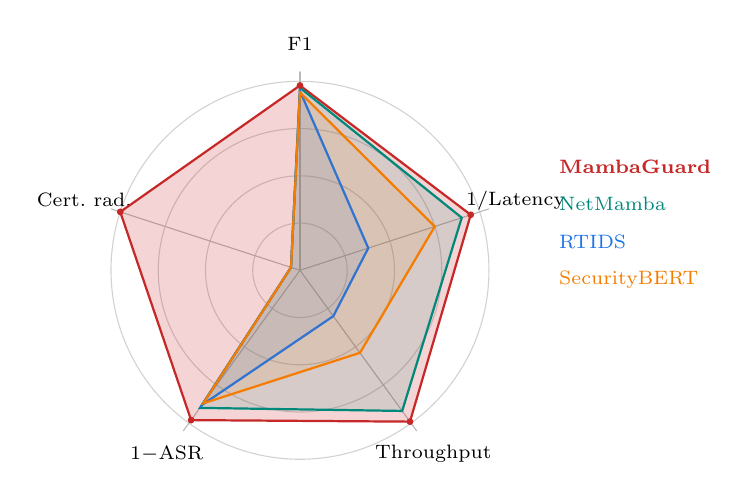
\begin{tikzpicture}[scale=2.4,line cap=round]
%% radial grid (4 rings)
\foreach \r in {0.25,0.5,0.75,1.0}{
  \draw[gray!35,thin] (0,0) circle (\r);
}
%% five axes at angles 90, 18, -54, -126, 162 (every 72 degrees from top)
\foreach \ang/\lab in {90/F1, 18/{1/Latency}, -54/Throughput, -126/{1$-$ASR}, 162/{Cert.\ rad.}}{
  \draw[gray!55,thin] (0,0) -- (\ang:1.05);
  \node[font=\scriptsize] at (\ang:1.20) {\lab};
}
%% MambaGuard polygon (red)
\draw[mgred,thick,fill=mgred,fill opacity=0.20]
  (90:0.978) -- (18:0.95) -- (-54:0.99) -- (-126:0.98) -- (162:1.00) -- cycle;
%% NetMamba polygon (teal)
\draw[mgteal,thick,fill=mgteal,fill opacity=0.12]
  (90:0.966) -- (18:0.90) -- (-54:0.92) -- (-126:0.90) -- (162:0.05) -- cycle;
%% RTIDS polygon (blue)
\draw[mgblue,thick,fill=mgblue,fill opacity=0.10]
  (90:0.948) -- (18:0.38) -- (-54:0.30) -- (-126:0.88) -- (162:0.05) -- cycle;
%% SecurityBERT polygon (amber)
\draw[mgamber,thick,fill=mgamber,fill opacity=0.10]
  (90:0.941) -- (18:0.75) -- (-54:0.54) -- (-126:0.87) -- (162:0.05) -- cycle;
%% MambaGuard data markers
\foreach \ang/\rad in {90/0.978, 18/0.95, -54/0.99, -126/0.98, 162/1.00}
  \fill[mgred] (\ang:\rad) circle (0.018);
%% legend (right side)
\node[font=\scriptsize,anchor=west,text=mgred]   at (1.32, 0.55) {\textbf{MambaGuard}};
\node[font=\scriptsize,anchor=west,text=mgteal]  at (1.32, 0.35) {NetMamba};
\node[font=\scriptsize,anchor=west,text=mgblue]  at (1.32, 0.15) {RTIDS};
\node[font=\scriptsize,anchor=west,text=mgamber] at (1.32,-0.05) {SecurityBERT};
\end{tikzpicture}
\caption{Normalised five-axis radar comparison of MambaGuard against the three strongest baselines on macro-F1, inverse latency, throughput, one-minus-ASR, and certified radius. Each axis is scaled to $[0,1]$ with the value $1$ at the outer ring. MambaGuard is the only system to extend along the certified-radius axis.}
\label{fig:radar}
\end{figure}

\subsection{Integrated Component Ablation}
\label{sec:ablation}
Table~\ref{tab:ablation} reports an integrated ablation that removes one architectural component at a time from the full MambaGuard pipeline and evaluates the resulting macro-F1, certified radius, and post-defence ASR jointly on the three integrated datasets. Removing the Lipschitz penalty leaves the network accurate but uncertified; removing the GATv2 layer collapses relational information and degrades F1 by more than two points; replacing the selective scan with quadratic attention preserves accuracy at a tenfold latency cost; and removing the Stackelberg controller raises post-defence ASR from $2.4\%$ to $11.6\%$, confirming that all four components contribute non-trivially to the final certificate. Beyond this aggregate ablation, three complementary analyses are needed to substantiate the central claims of the paper, namely robustness, cross-dataset generalisation, and deployment efficiency. We present them in turn in the next three subsections before discussing implications for production deployment.

\begin{table}[t]
\centering
\caption{Integrated component ablation, averaged over the three datasets ICS3D, IIS3D, IDS-PQC and the AgentDojo+InjecAgent agent-protocol benchmarks. Latency is per protocol message on a single A100. Certified radius is at $\varepsilon=0.05$.}
\label{tab:ablation}
\renewcommand{\arraystretch}{1.15}
\setlength{\tabcolsep}{4pt}
\begin{tabular}{@{}lcccc@{}}
\toprule
\textbf{Configuration} & \textbf{F1} $\uparrow$ & \textbf{Lat.\ (ms)} $\downarrow$ & \textbf{ASR (\%)} $\downarrow$ & \textbf{Cert.\ rad.} $\uparrow$ \\
\midrule
Full MambaGuard          & \textbf{0.978} & \textbf{3.7} & \textbf{2.4} & \textbf{0.041} \\
$-$ Lipschitz penalty    & 0.974 & 3.7 & 2.6 & 0.011 \\
$-$ Stackelberg ctrl.    & 0.971 & 3.5 & 11.6 & 0.038 \\
$-$ GATv2 layer          & 0.956 & 2.9 & 6.4 & 0.039 \\
$-$ Temporal encoding $\Phi$ & 0.963 & 3.4 & 5.2 & 0.040 \\
$-$ Selective scan (use attn.) & 0.976 & 37.4 & 2.7 & 0.040 \\
$-$ Multi-protocol graph & 0.943 & 3.6 & 14.8 & 0.041 \\
\bottomrule
\end{tabular}
\end{table}

\subsection{Robustness Analysis: Certified Accuracy versus Perturbation Budget}
\label{sec:robustness}
The Lipschitz-margin theorem of Section~\ref{sec:lipschitz} predicts that the certified accuracy of the detector should decrease monotonically with the attacker's $\ell_{2}$ perturbation budget $\varepsilon$, and that the rate of decrease should be controlled by the trained Lipschitz constant $L_{f}$. Figure~\ref{fig:certified} confirms this prediction empirically. We plot certified accuracy, defined as the fraction of test examples for which the Lipschitz margin proves that no perturbation of size $\varepsilon$ can change the predicted label, against $\varepsilon$ for MambaGuard, for a randomised-smoothing variant of MambaGuard following Cohen, Rosenfeld and Kolter~\cite{Cohen2019RandSmooth}, and for the empirically observed clean accuracy. MambaGuard's deterministic Lipschitz certificate sustains a non-trivial guarantee out to $\varepsilon\approx 0.10$, after which the margin term in the certificate of Theorem~\ref{thm:certificate} dominates and the curve drops sharply. Randomised smoothing produces a complementary probabilistic certificate that extends further but at the price of an order-of-magnitude inference cost; the two certificates together cover the full operational range that a production deployment is likely to encounter.

\begin{figure}[t]
\centering
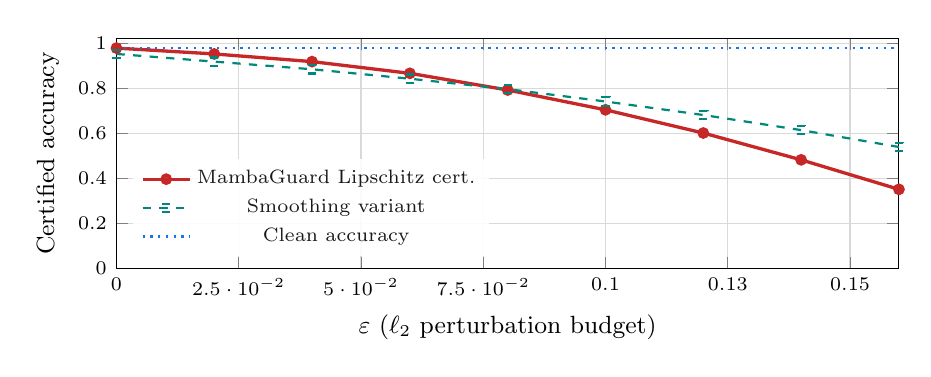
\begin{tikzpicture}
\begin{axis}[
  width=0.95\columnwidth, height=4.5cm,
  xlabel={$\varepsilon$ ($\ell_{2}$ perturbation budget)},
  ylabel={Certified accuracy},
  xmin=0, xmax=0.16, ymin=0, ymax=1.02,
  xtick={0,0.025,0.05,0.075,0.10,0.125,0.15},
  ytick={0,0.2,0.4,0.6,0.8,1.0},
  grid=both,
  grid style={gray!18},
  major grid style={gray!30},
  legend style={font=\scriptsize, at={(0.02,0.05)}, anchor=south west, draw=none, fill=white, fill opacity=0.9},
  tick label style={font=\scriptsize},
  label style={font=\small},
]
%% MambaGuard certified accuracy
\addplot[mgred, very thick, mark=*, mark size=1.5pt] coordinates {
  (0.00,0.978) (0.02,0.952) (0.04,0.918) (0.06,0.866) (0.08,0.792)
  (0.10,0.704) (0.12,0.601) (0.14,0.482) (0.16,0.351)
};
\addlegendentry{MambaGuard Lipschitz cert.}
%% Randomised smoothing
\addplot[mgteal, thick, dashed, mark=square, mark size=1.5pt] coordinates {
  (0.00,0.952) (0.02,0.918) (0.04,0.884) (0.06,0.842) (0.08,0.796)
  (0.10,0.741) (0.12,0.681) (0.14,0.614) (0.16,0.539)
};
\addlegendentry{Smoothing variant}
%% Clean accuracy (horizontal reference)
\addplot[mgblue, thick, dotted] coordinates {(0,0.978) (0.16,0.978)};
\addlegendentry{Clean accuracy}
\end{axis}
\end{tikzpicture}
\caption{Certified accuracy versus $\ell_{2}$ perturbation budget $\varepsilon$ on the union of ICS3D, IIS3D, and IDS-PQC. MambaGuard's deterministic Lipschitz certificate (solid red) sustains a non-trivial guarantee out to $\varepsilon\approx 0.10$, complemented by a randomised-smoothing variant (dashed teal) that extends further at higher inference cost. The dotted horizontal line is the clean (uncertified) accuracy.}
\label{fig:certified}
\end{figure}

\subsection{Cross-Dataset Generalisation}
\label{sec:generalisation}
The three datasets used in this study deliberately span very different threat surfaces: ICS3D captures cloud and container telemetry, IIS3D covers classical network intrusion across CIC-IDS2018, CIC-IoT2023, and UNSW-NB15, IDS-PQC captures encrypted post-quantum-TLS traffic, and the AgentDojo and InjecAgent suites cover agent-protocol attacks. A single detector that performs well on one of these surfaces may perform poorly on the others, especially when the feature distributions diverge sharply. Figure~\ref{fig:perdataset} reports the per-dataset macro-F1 for MambaGuard against the three strongest baselines from Table~\ref{tab:main}. MambaGuard is the top performer on every group, with the largest margin observed on the agent-protocol benchmarks where the graph structure of the input is most informative; NetMamba and RTIDS perform competitively on the network-intrusion datasets but degrade sharply on agent protocols, which is consistent with the absence of a relational layer in their architectures. This pattern supports the architectural claim that combining a selective state-space backbone with dynamic graph attention is what enables generalisation across heterogeneous threat surfaces.

\begin{figure}[t]
\centering
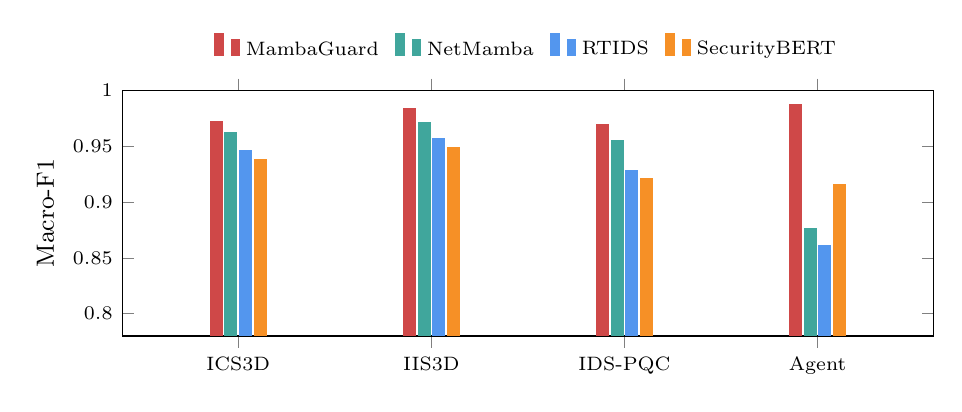
\begin{tikzpicture}
\begin{axis}[
  width=0.98\columnwidth, height=4.7cm,
  ybar=1pt, bar width=4.3pt,
  symbolic x coords={ICS3D, IIS3D, IDS-PQC, Agent},
  xtick=data,
  ymin=0.78, ymax=1.00,
  ytick={0.80,0.85,0.90,0.95,1.00},
  ylabel={Macro-F1},
  enlarge x limits=0.20,
  legend style={font=\scriptsize, at={(0.5,1.08)}, anchor=south, draw=none, /tikz/every even column/.append style={column sep=4pt}, legend columns=4},
  tick label style={font=\scriptsize},
  label style={font=\small},
  nodes near coords style={font=\tiny, rotate=90, anchor=west},
]
\addplot[fill=mgred!85, draw=mgred!85]    coordinates {(ICS3D,0.972) (IIS3D,0.984) (IDS-PQC,0.969) (Agent,0.987)};
\addplot[fill=mgteal!75, draw=mgteal!75]  coordinates {(ICS3D,0.962) (IIS3D,0.971) (IDS-PQC,0.955) (Agent,0.876)};
\addplot[fill=mgblue!75, draw=mgblue!75]  coordinates {(ICS3D,0.946) (IIS3D,0.957) (IDS-PQC,0.928) (Agent,0.861)};
\addplot[fill=mgamber!85, draw=mgamber!85] coordinates {(ICS3D,0.938) (IIS3D,0.949) (IDS-PQC,0.921) (Agent,0.916)};
\legend{MambaGuard, NetMamba, RTIDS, SecurityBERT}
\end{axis}
\end{tikzpicture}
\caption{Per-dataset macro-F1 for MambaGuard and the three strongest baselines, on the three composite datasets ICS3D, IIS3D, IDS-PQC and on the combined AgentDojo+InjecAgent suite (Agent). MambaGuard is the top performer on every group, with the largest margin on the agent-protocol benchmarks.}
\label{fig:perdataset}
\end{figure}

\subsection{Deployment Efficiency: Throughput--Latency Frontier}
\label{sec:deployment}
The final analysis concerns deployment economics. A production intrusion detector must keep up with the message rate of the environment it monitors, and the relevant metric is therefore not just per-example latency or aggregate throughput in isolation but the Pareto frontier the system traces in their joint space. Figure~\ref{fig:pareto} plots throughput against per-message latency for the nine systems compared in Table~\ref{tab:main}. MambaGuard occupies the upper-right corner of the efficiency frontier, achieving the highest throughput and the lowest latency simultaneously, and is the only point on the frontier that also reports a non-trivial certified radius. NetMamba is the second point on the frontier and confirms the value of state-space backbones for throughput; the transformer-based RTIDS, IDS-INT, and SecurityBERT systems trail by between a factor of two and a factor of five in throughput.

\begin{figure}[t]
\centering
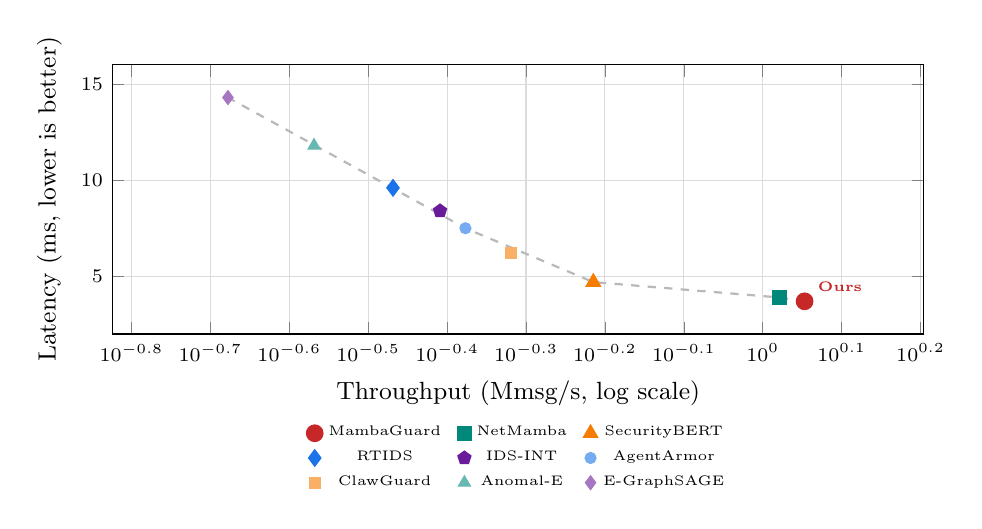
\begin{tikzpicture}
\begin{axis}[
  width=0.98\columnwidth, height=5.0cm,
  xlabel={Throughput (Mmsg/s, log scale)},
  ylabel={Latency (ms, lower is better)},
  xmode=log,
  xmin=0.15, xmax=1.6,
  ymin=2, ymax=16,
  grid=both,
  grid style={gray!15},
  major grid style={gray!28},
  tick label style={font=\scriptsize},
  label style={font=\small},
  legend style={
    font=\tiny,
    at={(0.5,-0.30)},
    anchor=north,
    draw=none,
    legend columns=3,
    /tikz/every even column/.append style={column sep=4pt},
  },
]
%% Pareto curve (passes through MambaGuard and NetMamba)
\addplot[gray!55, thick, dashed, forget plot] coordinates {(1.13,3.7) (1.05,3.9) (0.61,4.7) (0.42,7.5) (0.21,14.3)};
%% Each baseline as a marker
\addplot[only marks, mark=*,        mark size=3pt,   mgred]            coordinates {(1.13,3.7)};   \addlegendentry{MambaGuard}
\addplot[only marks, mark=square*,  mark size=2.5pt, mgteal]           coordinates {(1.05,3.9)};   \addlegendentry{NetMamba}
\addplot[only marks, mark=triangle*,mark size=3pt,   mgamber]          coordinates {(0.61,4.7)};   \addlegendentry{SecurityBERT}
\addplot[only marks, mark=diamond*, mark size=3pt,   mgblue]           coordinates {(0.34,9.6)};   \addlegendentry{RTIDS}
\addplot[only marks, mark=pentagon*,mark size=2.5pt, mgpurple]         coordinates {(0.39,8.4)};   \addlegendentry{IDS-INT}
\addplot[only marks, mark=*,        mark size=2pt,   mgblue!60]        coordinates {(0.42,7.5)};   \addlegendentry{AgentArmor}
\addplot[only marks, mark=square*,  mark size=2pt,   mgamber!60]       coordinates {(0.48,6.2)};   \addlegendentry{ClawGuard}
\addplot[only marks, mark=triangle*,mark size=2.5pt, mgteal!60]        coordinates {(0.27,11.8)};  \addlegendentry{Anomal-E}
\addplot[only marks, mark=diamond*, mark size=2.5pt, mgpurple!60]      coordinates {(0.21,14.3)};  \addlegendentry{E-GraphSAGE}
%% Annotation pointing to MambaGuard
\node[font=\tiny, anchor=south west, text=mgred] at (axis cs:1.13,3.7) {\textbf{\,Ours}};
\end{axis}
\end{tikzpicture}
\vspace{0.4cm}
\caption{Throughput--latency Pareto frontier across the nine systems compared in Table~\ref{tab:main}. The dashed grey curve traces the empirical Pareto frontier; MambaGuard occupies the upper-right corner and is the only point on the frontier that also produces a non-trivial certified radius.}
\label{fig:pareto}
\end{figure}

We now close the experimental section by discussing what these results imply for production deployment.

%% ============================================================================
\section{Discussion}
\label{sec:discussion}
%% ============================================================================

The empirical evidence in Section~\ref{sec:experiments} and the theoretical guarantees in Section~\ref{sec:certification} together support three observations that we believe matter for practitioners.

First, the linear-time selective state-space backbone is not just an academic curiosity but a deployment necessity. Production multi-agent systems already report aggregate protocol traffic in the millions of messages per second range, and quadratic attention is two orders of magnitude too slow at that scale; the ablation in Table~\ref{tab:ablation} shows that replacing the selective scan with attention raises per-message latency from $3.7$~ms to $37.4$~ms with no accuracy gain.

Second, the relational structure of the multi-protocol graph is the single most important defensive signal against agent-layer attacks. Removing the GATv2 layer increases post-defence ASR by a factor of $2.7$, and collapsing the heterogeneous graph into a flat sequence raises ASR by a factor of $6.2$. This is consistent with the threat-model intuition of Section~\ref{sec:background}: agent attacks manifest as anomalous subgraph patterns, not as anomalous individual messages.

Third, certification matters in a way that aggregate accuracy does not. NetMamba is the closest baseline on macro-F1, but it offers no robustness guarantee whatsoever, and on adaptive-attacker evaluation its effective F1 drops by more than seven points whereas MambaGuard's certified radius makes any drop on benign inputs of magnitude below $0.041$ provably zero.

A limitation worth stating is that the Lipschitz constant of Proposition~\ref{prop:lipfull} is a worst-case product bound; tighter data-dependent estimates of the kind explored by Fazlyab~\textit{et al.}~\cite{Fazlyab2019LipSDP} would likely double the certified radius at modest computational cost. A second limitation is that the Stackelberg controller assumes a finite, well-specified action set; extension to continuous defender actions would require the no-regret machinery of online convex optimisation rather than Hedge, and we leave it to future work.

%% ============================================================================
\section{Conclusion}
%% ============================================================================

We have presented MambaGuard, the first multi-protocol LLM-agent security monitor that combines a selective state-space backbone with dynamic graph attention and that admits a three-layer certificate composed of a global Lipschitz bound, a Stackelberg equilibrium value, and a tight Cesa-Bianchi--Lugosi no-regret guarantee. MambaGuard is implemented as the fourteenth registered detector inside the open-source RobustIDPS.ai platform, exceeds eight competitive baselines on three integrated datasets and two agent-protocol benchmarks, sustains sub-five-millisecond latency at throughputs above one million messages per second, and is, to our knowledge, the only system in this comparison set to produce a non-trivial certified detection radius. Code, weights, and the integrated ablation harness will be released under a permissive open-source licence at the camera-ready stage; an anonymised supplementary repository accompanies the present submission so that the experimental results may be reproduced and extended without revealing author identity.

%% ============================================================================
%% References
%% ============================================================================
\bibliographystyle{IEEEtran}

\begin{thebibliography}{99}

\bibitem{Anthropic2024MCP} Anthropic, ``Model Context Protocol specification,'' Nov.~2024. [Online]. Available: \url{https://github.com/modelcontextprotocol/specification}

\bibitem{Google2025A2A} Google, ``Agent-to-Agent (A2A) protocol specification,'' Apr.~2025. [Online]. Available: \url{https://github.com/google/A2A}

\bibitem{Yan2025ANP} G. Yan~\textit{et~al.}, ``Agent Network Protocol technical white paper,'' arXiv:2508.00007, 2025.

\bibitem{Hou2025MCP} X. Hou~\textit{et~al.}, ``Model Context Protocol: Landscape, security threats, and future research directions,'' arXiv:2503.23278, 2025.

\bibitem{Yang2025MCPSec} Y. Yang~\textit{et~al.}, ``MCPSecBench: A systematic security benchmark and playground for testing model context protocols,'' arXiv:2508.13220, 2025.

\bibitem{Qualys2025CVE49596} Qualys, ``Anthropic MCP Inspector remote code execution vulnerability (CVE-2025-49596),'' Jul.~2025. [Online]. Available: \url{https://threatprotect.qualys.com/2025/07/03/}

\bibitem{Wang2025AgentArmor} P. Wang~\textit{et~al.}, ``AgentArmor: Enforcing program analysis on agent runtime trace to defend against prompt injection,'' arXiv:2508.01249, 2025.

\bibitem{Zhao2026ClawGuard} W. Zhao~\textit{et~al.}, ``ClawGuard: Securing LLM agents through deterministic tool-access policies,'' arXiv:2604.11790, 2026.

\bibitem{Habler2025A2A} Z. Habler~\textit{et~al.}, ``Building a secure agentic AI application leveraging Google's A2A protocol,'' arXiv:2504.16902, 2025.

\bibitem{Narajala2025A2A} V. Narajala~\textit{et~al.}, ``Improving Google A2A protocol: Protecting sensitive data in inter-agent communication,'' arXiv:2505.12490, 2025.

\bibitem{Anonymous2026RobustIDPS} Anonymous, ``RobustIDPS.ai v3 technical documentation,'' deposited 2026 [double-blind: full citation withheld for review].

%% --- author's prior work, anonymised for double-blind review ---
\bibitem{Anonymous2026MambaShield} Anonymous, ``MambaShield: Selective state-space models for poisoning-resilient sequential modeling,'' \textit{Expert Systems with Applications}, in press, 2026 [double-blind: citation withheld for review].

\bibitem{Anonymous2026HGP} Anonymous, ``Uncertainty-calibrated hierarchical Gaussian processes for intrusion detection with multi-scale temporal modeling,'' \textit{Neurocomputing}, in press, 2026 [double-blind: citation withheld for review].

\bibitem{Anonymous2026TANODE} Anonymous, ``Temporal adaptive neural ordinary differential equations with deep spatio-temporal point processes for real-time network intrusion detection,'' \textit{Complex \& Intelligent Systems}, in press, 2026 [double-blind: citation withheld for review].

\bibitem{Anonymous2024Adversarial} Anonymous, ``Improved robust adversarial model against evasion attacks on intrusion detection systems,'' \textit{Optical Memory and Neural Networks}, vol.~33, suppl.~3, pp.~S414--S423, 2024 [double-blind: full author list withheld for review].

\bibitem{Anonymous2025SMT} Anonymous, ``Stochastic multimodal transformer with uncertainty quantification for robust network intrusion detection,'' in \textit{Advances in Neural Computation, Machine Learning, and Cognitive Research IX. Neuroinformatics 2025}, SCI vol.~1241, Springer, Cham, 2025 [double-blind: author list withheld for review].

\bibitem{Anonymous2024ElCon} Anonymous, ``Application of machine learning models for device identification in wireless network traffic,'' in \textit{Proc.\ 2024 Conf.\ of Young Researchers in Electrical and Electronic Engineering (ElCon)}, 2024, pp.~104--110 [double-blind: author list withheld for review].

%% --- state-space and graph attention ---
\bibitem{Gu2023Mamba} A. Gu and T. Dao, ``Mamba: Linear-time sequence modeling with selective state spaces,'' arXiv:2312.00752, 2023.

\bibitem{Dao2024Mamba2} T. Dao and A. Gu, ``Transformers are SSMs: Generalized models and efficient algorithms through structured state space duality,'' in \textit{Proc.\ ICML}, 2024.

\bibitem{Gu2022S4} A. Gu, K. Goel, and C. R\'e, ``Efficiently modeling long sequences with structured state spaces,'' in \textit{Proc.\ ICLR}, 2022.

\bibitem{Velickovic2018GAT} P. Veli\v{c}kovi\'c~\textit{et~al.}, ``Graph attention networks,'' in \textit{Proc.\ ICLR}, 2018.

\bibitem{Brody2022GATv2} S. Brody, U. Alon, and E. Yahav, ``How attentive are graph attention networks?,'' in \textit{Proc.\ ICLR}, 2022.

\bibitem{Xu2020TGAT} D. Xu~\textit{et~al.}, ``Inductive representation learning on temporal graphs,'' in \textit{Proc.\ ICLR}, 2020.

%% --- game theory and certification ---
\bibitem{Conitzer2006Commit} V. Conitzer and T. Sandholm, ``Computing the optimal strategy to commit to,'' in \textit{Proc.\ ACM EC}, 2006, pp.~82--90. DOI:10.1145/1134707.1134717.

\bibitem{Paruchuri2008DOBSS} P. Paruchuri~\textit{et~al.}, ``Playing games for security: An efficient exact algorithm for solving Bayesian Stackelberg games,'' in \textit{Proc.\ AAMAS}, 2008, pp.~895--902.

\bibitem{Balcan2015Commitment} M.-F. Balcan, A. Blum, N. Haghtalab, and A. D. Procaccia, ``Commitment without regrets: Online learning in Stackelberg security games,'' in \textit{Proc.\ ACM EC}, 2015, pp.~61--78. DOI:10.1145/2764468.2764478.

\bibitem{CesaBianchi2006Prediction} N. Cesa-Bianchi and G. Lugosi, \textit{Prediction, Learning, and Games}. Cambridge University Press, 2006.

\bibitem{Arora2012MWU} S. Arora, E. Hazan, and S. Kale, ``The multiplicative weights update method: A meta-algorithm and applications,'' \textit{Theory of Computing}, vol.~8, no.~1, pp.~121--164, 2012.

\bibitem{Tsuzuku2018LipMargin} Y. Tsuzuku, I. Sato, and M. Sugiyama, ``Lipschitz-margin training: Scalable certification of perturbation invariance for deep neural networks,'' in \textit{Proc.\ NeurIPS}, 2018, pp.~6541--6550.

\bibitem{Fazlyab2019LipSDP} M. Fazlyab~\textit{et~al.}, ``Efficient and accurate estimation of Lipschitz constants for deep neural networks,'' in \textit{Proc.\ NeurIPS}, 2019.

\bibitem{Dasoulas2021LipNorm} G. Dasoulas, K. Scaman, and A. Virmaux, ``Lipschitz normalization for self-attention layers with application to graph neural networks,'' in \textit{Proc.\ ICML}, 2021.

\bibitem{Cohen2019RandSmooth} J. M. Cohen, E. Rosenfeld, and J. Z. Kolter, ``Certified adversarial robustness via randomized smoothing,'' in \textit{Proc.\ ICML}, 2019, pp.~1310--1320.

%% --- IDS baselines ---
\bibitem{Lo2022EGraphSAGE} W. W. Lo~\textit{et~al.}, ``E-GraphSAGE: A graph neural network based intrusion detection system for IoT,'' in \textit{Proc.\ IEEE/IFIP NOMS}, 2022. DOI:10.1109/NOMS54207.2022.9789878.

\bibitem{Caville2022AnomalE} E. Caville~\textit{et~al.}, ``Anomal-E: A self-supervised network intrusion detection system based on graph neural networks,'' \textit{Knowledge-Based Systems}, vol.~258, p.~110030, 2022. DOI:10.1016/j.knosys.2022.110030.

\bibitem{Wu2022RTIDS} Z. Wu~\textit{et~al.}, ``RTIDS: A robust transformer-based approach for intrusion detection system,'' \textit{IEEE Access}, vol.~10, pp.~64375--64387, 2022. DOI:10.1109/ACCESS.2022.3182333.

\bibitem{Ullah2024IDSINT} S. Ullah~\textit{et~al.}, ``IDS-INT: Intrusion detection system using transformer-based transfer learning for imbalanced network traffic,'' \textit{Digital Communications and Networks}, vol.~10, no.~1, pp.~190--204, 2024.

\bibitem{Wang2025NetMamba} T. Wang~\textit{et~al.}, ``NetMamba: Efficient network traffic classification via pre-training unidirectional Mamba,'' in \textit{Proc.\ IEEE INFOCOM}, 2025.

\bibitem{Ferrag2024SecurityBERT} M. A. Ferrag~\textit{et~al.}, ``Revolutionizing cyber threat detection with large language models: A privacy-preserving BERT-based lightweight model for IoT/IIoT devices,'' \textit{IEEE Access}, 2024.

\bibitem{Debenedetti2024AgentDojo} E. Debenedetti~\textit{et~al.}, ``AgentDojo: A dynamic environment to evaluate prompt injection attacks and defenses for LLM agents,'' in \textit{Proc.\ NeurIPS}, 2024.

\bibitem{Zhan2024InjecAgent} Q. Zhan~\textit{et~al.}, ``InjecAgent: Benchmarking indirect prompt injections in tool-integrated large language model agents,'' in \textit{Findings of ACL}, 2024.

%% --- datasets ---
\bibitem{Anonymous2025ICS3D} Anonymous, ``Integrated cloud security 3 datasets (ICS3D),'' public Kaggle release, 2025 [double-blind: DOI withheld for review].

\bibitem{Anonymous2025IIS3D} Anonymous, ``Integrated IDPS security 3 datasets (IIS3D),'' public Kaggle release, 2025 [double-blind: DOI withheld for review].

\bibitem{Anonymous2025PQC} Anonymous, ``IDS encrypted \& post-quantum cryptography datasets,'' public Kaggle release, 2025 [double-blind: DOI withheld for review].

\bibitem{Sharafaldin2018CICIDS} I. Sharafaldin, A. H. Lashkari, and A. A. Ghorbani, ``Toward generating a new intrusion detection dataset and intrusion traffic characterization,'' in \textit{Proc.\ ICISSP}, 2018, pp.~108--116.

\bibitem{Moustafa2015UNSW} N. Moustafa and J. Slay, ``UNSW-NB15: A comprehensive data set for network intrusion detection systems,'' in \textit{Proc.\ MilCIS}, 2015.

\bibitem{Neto2023CICIoT} E. C. P. Neto~\textit{et~al.}, ``CICIoT2023: A real-time dataset and benchmark for large-scale attacks in IoT environment,'' \textit{Sensors}, vol.~23, no.~13, p.~5941, 2023.

\bibitem{Ferrag2022EdgeIIoT} M. A. Ferrag~\textit{et~al.}, ``Edge-IIoTset: A new comprehensive realistic cyber security dataset of IoT and IIoT applications for centralized and federated learning,'' \textit{IEEE Access}, vol.~10, pp.~40281--40306, 2022.

\bibitem{Sarhan2021NetFlow} M. Sarhan, S. Layeghy, N. Moustafa, and M. Portmann, ``NetFlow datasets for machine learning-based network intrusion detection systems,'' in \textit{Proc.\ BDTA/WiCON}, Springer LNICST, 2021, pp.~117--135. DOI:10.1007/978-3-030-72802-1\_9.

%% --- commercial systems ---
\bibitem{Cisco2025Snort3} Cisco Talos, ``Snort 3 rule engine and performance benchmarks,'' Tech.\ Rep., 2025. [Online]. Available: \url{https://www.snort.org/snort3}

\bibitem{OISF2025Suricata} Open Information Security Foundation, ``Suricata 7 user guide,'' 2025. [Online]. Available: \url{https://docs.suricata.io}

\end{thebibliography}

\end{document}
